\documentclass{book}
\usepackage{hyperref}
\usepackage{amsmath}
\usepackage{multicol}
\usepackage[dvipsnames]{xcolor}
\usepackage{graphicx}
\usepackage{subcaption}
\usepackage{changepage}
\usepackage[spanish]{babel}
\begin{document}
\setcounter{chapter}{1}

\chapter*{Tratamiento de datos}

En este capítulo se recoge un breve resumen de tratamiento y representación de datos,
con los elementos fundamentales necesarios para la elaboración de informes del curso.

\section{Expresión de resultados}

Una medición nos permite determinar un valor asociado a una magnitud física, bien mediante
la cuenta de un número de sucesos o comparación con una unidad de medida. Cuando realizamos
una medición es imposible determinar el valor exacto de dicha magnitud, por lo que debemos
limitarnos a encontrar un valor aproximado siempre limitado por la precisión de los instrumentos
de medida y el observador, así como las propiedades intrínsecas de la materia (fluctuaciones,
indeterminación, etc). De esta manera, cuando realizamos sucesivas medidas podemos obtener valores
ligeramente distintos, y esto nos obliga a presentar nuestros resultados dando un valor estimado dentro
de un rango en el que tenemos un grado de confianza en el que se encuentra el valor verdadero de
la magnitud. Esto es, toda magnitud física derivada de un experimento lleva asociado un error, 
que ha de expresarse siempre junto al valor estimado, normalmente mediante el símbolo '$\pm$'.
Sea una magnitud $x$, denotaremos su error asociado como $\Delta x$. Veamos un ejemplo:


\begin{equation}
    m = 5.64 \pm 0.23 \; \mathrm{kg}
\end{equation}

Destacamos varios puntos sobre la representación de este error asociado:

\begin{itemize}
  \item Todos los resultados presentes en un informe de laboratorio deben incluir su error 
  asociando.
  \item Todos los resultados deben expresarse junto a las \textbf{unidades} en las que se mide dicha 
  magnitud física.
  \item Todo error tiene como \textbf{máximo dos cifras significativas}. Además, la cantidad medida
  ha de tener como última cifra significativa la última de su error. No tiene sentido proporcionar
  un valor con más precisión que el error (Ver ejemplos a continuación.)
  \item Frecuentemente, las variables se representan con letra formateada cursiva, mientras 
  que para las unidades se emplea un formato regular.
\end{itemize}

A continuación se muestran algunos ejemplos de buena y mala representación de resultados medidos.

\begin{equation}
  \begin{aligned}
    & \color{ForestGreen} P = 14800 \pm 3000 \; \mathrm{Pa} \\
    & \color{ForestGreen} \rho = 7860.1 \pm 2.3 \; \mathrm{kg / m^{-3}} \\
    & \color{ForestGreen} v = 2300 \pm 700 \; \mathrm{m/s} \\
    & \color {ForestGreen} d = ( 23.21 \pm 75 ) \pm 10^{-6} \; \mathrm{\mu m}
  \end{aligned}
\end{equation}

\begin{equation}
  \begin{aligned}
    & \color{Red} P = 14845 \pm 3253 \; \mathrm{Pa} \\
    & \color{Red} \rho = 7860.1 \pm 2.3 \; kg / m^{-3} \\
    & \color{Red} v = 2336 \pm 700 \; \mathrm{m/s} \\
    & \color {Red} d = ( 23.2186 \pm 7506 ) \pm 10^{-6} \; \mathrm{\mu m}
  \end{aligned}
\end{equation}


Es muy importante representar los resultados correctamente. Un informe nunca podrá obtener una
buena calificación si hay fallos en este aspecto. Como norma general, se recomienda trabajar con
unidades del sistema internacional y sus múltiplos para evitar errores derivados del manejo de
unidades.

En las siguientes secciones se detalla cómo calcular el error asociado a una magnitud física. 
Este error se obtendrá de forma diferente dependiendo de si el valor se observa directamente en
instrumento de medida (\textbf{medida directa}) o si se obtiene utilizando expresiones matemáticas a partir
de una o varias medidas directas (\textbf{medida indirecta}).


\section{Incertidumbre en medidas directas}
Esta incertidumbre se asocia con la medida directa de una magnitud mediante un dispositivo o técnica.
Dentro de esta incertidumbre, encontramos contribuciones de distinto tipo que debemos considerar
en su conjunto.
\subsection{Tipo A}
También conocido como incertidumbre estadística. Se asocia con factores ambientales aleatorios, 
fluctuaciones o vibraciones. Por ejemplo, variaciones de temperatura a lo largo de un experimento.
Para determinar esta contribución al error debemos realizar $n$ medidas, y se calcula su desviación
típica $s$. La magnitud tomará el valor medio de estas $n$ medidas, y el error asociado de tipo A 
vendrá determinado por:

\begin{equation}
  \Delta x_A = \frac{s}{\sqrt{n}}
\end{equation}

\textcolor{red}{¿Incluimos multiplicar por la t de student o preferís no hacerlo?}

\subsection{Tipo B}
También conocida como incertidumbre sistemática de precisión, se relaciona con la sensibilidad,
denotada como $\delta x$, del instrumento utilizado. Así, el error tipo B se corresponderá con:

\begin{equation}
  \Delta x_B = \delta x
\end{equation}

En caso de no disponer de ninguna referencia, suele tomarse su valor como una unidad de la cifra 
que se puede apreciar con el aparato. Sin embargo, el error instrumental suele ser mayor que esta 
última cifra y muchos fabricantes así lo indican en los manuales de uso de los dispositivos. Por 
tanto es necesario consultar siempre si el instrumento que estamos utilizando dispone de alguna 
indicación de su precisión.

Un ejemplo muy claro es el caso de los polímetros, en los que siempre se dispone de un manual en
el que el fabricante detalla el error instrumental asociado a cada magnitud como un tanto por
ciento de la medida más algunos dígitos. Por ejemplo, supongamos que medimos un volataje y
la pantalla del polímetro muestra $23.85 \; \textrm{V}$. Si recurrimos al manual encontraremos que la precisión
del aparato para el voltaje es de un 1\% del valor leído + 3 dígitos. Por tanto, el error de tipo
B asociado a esta medida será

\begin{equation}
  \Delta x_B = 0.24 \pm 0.03 \; \textrm{V} = 0.27 \; \textrm{V}
\end{equation}

\subsection{Incertidumbre combinada y otras contribuciones}

Las dos contribuciones anteriores han de considerarse para el cálculo del error total asociado a
una media. Es por ello que se define la incertidumbre combinada como la suma cuadrática de las
incertidumbres de tipo A y B.

\begin{equation}
  \Delta x_C = \sqrt{(\Delta x_A)^2 + (\Delta x_B)^2}
\end{equation}

No obstante, existen otras causas distintas a las anteriores que pueden degradar una medida, y
que agrupamos bajo el nombre de \textbf{incertidumbre sistemática}. Estas son incertidumbres que se producen
en cada medida de la magnitud que se realiza, y que pueden deberse a una mala interpretación de
los valores proporcionados por el dispositivo o a un error de calibración (error de cero) que
desplace o distorsione la medida. Hemos de asegurarnos antes de comenzar la toma de datos que no
estamos incurriendo en ningún error de este tipo.

\section{Incertidumbre en medidas indirectas}

Una vez obtenidas las incertidumbres de las medidas directas, si queremos determinar cualquier
magnitud derivada, debemos obtener el error de esta medida indirecta. Supongamos una medida
indirecta $y$ que se obtiene a partir de varias medidas directas independientes $x_1$, $x_2$, 
... $x_n$  y una serie de constntes $c_1$, $c_2$, ... $c_m$, mediante una relación funcional:

\begin{equation}
  y = f(x_1, x_2, ... c_1, c_2, ...)
\end{equation}

El valor esperado de esta magnitud indirecta $y$ se calcula a partir de los valores medidos:

\begin{equation}
  \bar{y} = f(\bar{x}_1, \bar{x}_2, ... c_1, c_2, ...)
\end{equation}

La incertidumbre de esta magnitud $y$ se obtiene de la llamada \textbf{propagación cuadrática de 
errores}.

\begin{equation}
  \Delta y = \sqrt{ \left( \frac{\partial f}{\partial x_1} \right)^2 (\Delta_C x_1)^2 + 
  \left( \frac{\partial f}{\partial x_2} \right)^2 (\Delta_C x_2)^2 + ... +
  \left( \frac{\partial f}{\partial x_n} \right)^2 (\Delta_C x_n)^2}
\end{equation}

Respecto a las constantes, debemos de asegurarnos de tomar sus valores con la suficiente precisión
como para que su contribución a la incertidumbre pueda considerarse despreciable. Algunos casos
frecuentes de propagación cuadrática de errores se detallan a continuación.

\begin{center}
  \renewcommand{\arraystretch}{1.75}
  \begin{tabular}{lll}
    Cambio de ecala & $y = c x$ & $\Delta y = | c \Delta x |$  \\
    Potencias & $y = c x^b$ & $\Delta y = | b c x^{b-1} \Delta x|$ \\
    Suma y diferencia & $y = x_1 \pm x_2$ & $\Delta y = \sqrt{(\Delta x_1)^2 + (\Delta x_2)^2}$ \\
    Producto & $y = x_1 \cdot x_2$ & $\Delta y = \sqrt{(x_2 \Delta x_1)^2 + (x_1 \Delta x_2)^2}$ \\ 
  \end{tabular} 
\end{center}


\section{Ajustes y representaciones}

En numerosas experiencias de laboratorio se pedirá comprobar ciertas leyes mediante la realización
de algún experimento. Es decir, ha de demostrarse que existe una relación funcional entre dos
magnitudes. Una manera especialmente útil de demostrar esta relación es mediante ajustes, buscando
la expresión matemática que mejor aproxime la relación entre dos variables $y$ y $x$.

Para hallar esta expresión utilizaremos el método de los mínimos cuadrados, en el que se optimizan
los parámetros libres de la función de forma que el error cuadrático (diferencia entre los valores
medidos y los previstos, al cuadrado) sea mínimo.

Siempre que sea posible, utilizaremos un ajuste lineal, es decir, utilizando variables entre las
que se prevea una relación lineal. 

\begin{equation}
  y = m x + c ,
\end{equation}

donde $m$ y $c$ son dos parámetros de ajuste. Si la ley que queremos demostrar no prevee una 
relación lineal
entre variables, deberemos intentar linearizar la relación. Supongamos, por ejemplo, dos magnitudes
relacionadas mediante una ley de Potencias

\begin{equation}
  y = c x^b
\end{equation}

En el laboratorio mediremos valores de $x$ e $y$, y para demostrar si existe la relación prevista
entre ambas magnitudes realizaremos un ajuste por mínimos cuadrados. Para poder realizar un ajuste
lineal de este conjunto de medidas, podemos linearizar la ecuación tomando logaritmos:

\begin{equation}
  \log{y} = b \log{x} + \log{c}
\end{equation}

De esta manera, trabajando con los logaritmos de las magnitudes medidas podemos hallar los 
parámetros de ajuste mediante un ajuste lineal. La pendiente de esta recta nos dará el exponente
y el corte con el eje de ordenadas el logaritmo de la constante multiplicativa de la relación
original.

Por supuesto no siempre es posible obtener una expresión lineal entre dos magnitudes que se
desean relacionar, por lo que habrá casos en los que tengamos que realizar ajustes no lineales.
Los programas generalmente utilizados (Gnuplot, Origin, Mathematica, Python ...) siempre ofrecen
la posibilidad de ajustes no lineales.

Es muy importante tener presente que sea cual sea la dependencia funcional, \textbf{los parámetros de
ajuste siempre han de presentarse junto a su error}, de forma que podamos realizar propagación
cuadrática para obtener los errores de magnitudes derivadas. Los programas de ajuste mencionados
suelen ofrecer el error de los parámetros, normalmente en un intervalo de estimación del 95\%.


\subsection{Test de bondad del ajuste}

Siempre que se realice un ajuste funcional a los datos experimentales es necesario realizar un
test de bondad para comprobar si este ajuste es significativo y realmente explica la dependencia
propuesta para los valores medidos. Existen numerosas maneras de medir la calidad del ajuste, entre
los que podemos señalar:

\begin{itemize}
  \item \textbf{Coeficiente de correlación.} Normalmente denotado con $r$, suele ser proporcionado
  por el propio software de ajuste, con un valor que oscila entre $-1$ (ajuste perfecto con
  pendiente negativa) y $1$ (ajuste perfecto con pendiente positiva). Valores cercanos a $0$ 
  indican que no existe correlación entre los valores medidos y la función propuesta.
  También es usual proporcionar el coeficiente de correlación $R^2$, que para un ajuste lineal 
  coincide con el cuadrado de $r$.
  \item \textbf{Test chi-cuadrado.} Se obtiene del programa de ajuste o se calcula el valor
  experimental de $\chi^2$
  \begin{equation}
    \chi_{\textrm{exp}}^2 = \sum_{i=1}^n \frac{(y_i^{\textrm{obs}} - y_i^{\textrm{ajuste}})^2}{(\Delta y_i^{\textrm{obs}})^2}
  \end{equation}
  Este valor ha de compararse con el tabulado con $n-p$ grados de libertad,
  donde $p$ es el número de grupos medidos y $n$ el número total de muestas.
  \item \textbf{F de Fisher.} El valor experimental que proporciona el programa de ajuste se compara
  con el tabulado, usando por norma general un 95\% de confianza y grados de libertad $(p-1, n-p)$.
\end{itemize}


\subsection{Representación gráfica}
Para garantizar que las representaciones gráficas sean inteligibles y útiles, han de realizarse 
siguiendo una serie de pautas de buenas prácticas:

\begin{itemize}
  \item Procura elegir adecuadamente las escalas de los ejes, de forma que los valores queden
  ajustados dentro de la caja de la gráfica.
  \item Indicar la magnitud representada y sus unidades en cada eje. Utiliza siempre un formato y
  tamaño adecuado para que puedan leerse correctamente.
  \item Mostrar los datos experimentales junto con sus barras de error siempre que sea posible.
  \item Distinguir mediante distintos símbolos y/o colores los distintos conjuntos de datos,
  procurando mantener una leyendas legible en la que se indique qué representa cada conjunto.
  \item Es recomendable incluir un pie de figura en el que se den detalles sobre la representación.
  \item No unir mediante segmentos los datos que se representen en las gráficas. Los datos obtenidos
  en el laboratorio se corresponden generalmente con medidas discretas, por lo que habrán de representarse
  mediante símbolos y nunca con líneas. Las líneas han de usarse para representar las funciones de
  ajuste.
\end{itemize}

En la Figura \ref{fig:dosgrafs} se muestran dos ejemplos de mala y buena representación 
respectivamente para el mismo conjunto de datos.

\begin{figure}[h]
  
  \begin{adjustwidth}{-3cm}{-4.5cm}
  \centering
  \begin{subfigure}{0.45\pdfpagewidth}
      \centering
      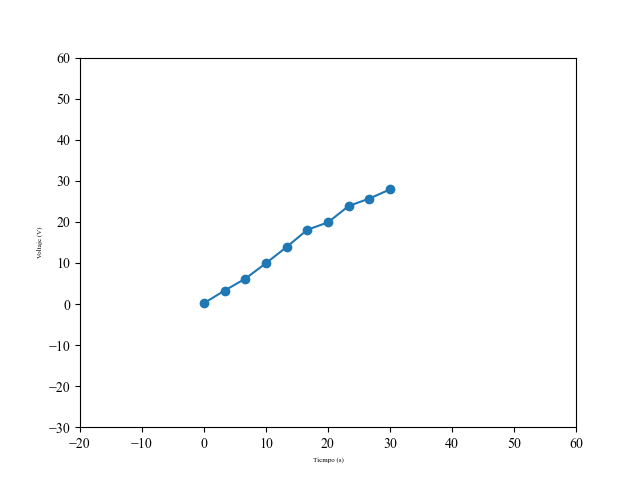
\includegraphics[width=\linewidth]{assets/fig/malagrafica.png}
      \caption{}
      \label{fig:malagraf}
  \end{subfigure}
  \hfill
  \begin{subfigure}{0.45\pdfpagewidth}
      \centering
      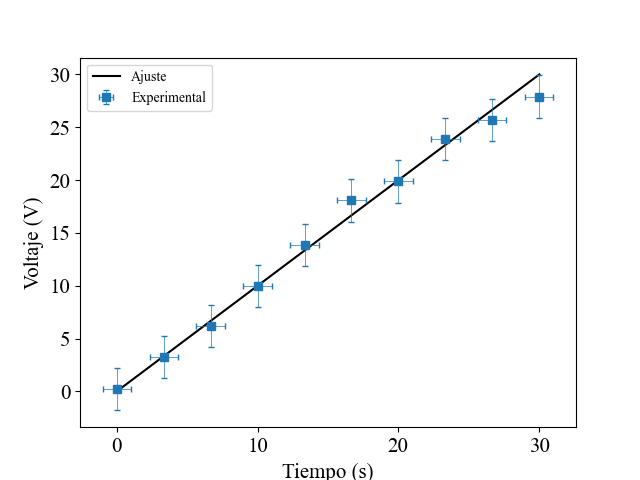
\includegraphics[width=\linewidth]{assets/fig/buenagrafica.png}
      \caption{}
      \label{fig:buenagraf}
  \end{subfigure}
  \end{adjustwidth}
  \caption{Dos representaciones del mismo conjunto de datos. (a) representa un fatal
  ejemplo de representación. (b) muestra los mismos datos junto a un ajuste lineal
  de una manera mucho más clara.}
  \label{fig:dosgrafs}
  
\end{figure}




\end{document}